\documentclass[]{article}
\usepackage{lmodern}
\usepackage{amssymb,amsmath}
\usepackage{ifxetex,ifluatex}
\usepackage{fixltx2e} % provides \textsubscript
\ifnum 0\ifxetex 1\fi\ifluatex 1\fi=0 % if pdftex
  \usepackage[T1]{fontenc}
  \usepackage[utf8]{inputenc}
\else % if luatex or xelatex
  \ifxetex
    \usepackage{mathspec}
  \else
    \usepackage{fontspec}
  \fi
  \defaultfontfeatures{Ligatures=TeX,Scale=MatchLowercase}
\fi
% use upquote if available, for straight quotes in verbatim environments
\IfFileExists{upquote.sty}{\usepackage{upquote}}{}
% use microtype if available
\IfFileExists{microtype.sty}{%
\usepackage{microtype}
\UseMicrotypeSet[protrusion]{basicmath} % disable protrusion for tt fonts
}{}
\usepackage[margin=0.1in]{geometry}
\usepackage{hyperref}
\hypersetup{unicode=true,
            pdftitle={STAT565\_Lab},
            pdfauthor={Shen Qu},
            pdfborder={0 0 0},
            breaklinks=true}
\urlstyle{same}  % don't use monospace font for urls
\usepackage{color}
\usepackage{fancyvrb}
\newcommand{\VerbBar}{|}
\newcommand{\VERB}{\Verb[commandchars=\\\{\}]}
\DefineVerbatimEnvironment{Highlighting}{Verbatim}{commandchars=\\\{\}}
% Add ',fontsize=\small' for more characters per line
\usepackage{framed}
\definecolor{shadecolor}{RGB}{248,248,248}
\newenvironment{Shaded}{\begin{snugshade}}{\end{snugshade}}
\newcommand{\AlertTok}[1]{\textcolor[rgb]{0.94,0.16,0.16}{#1}}
\newcommand{\AnnotationTok}[1]{\textcolor[rgb]{0.56,0.35,0.01}{\textbf{\textit{#1}}}}
\newcommand{\AttributeTok}[1]{\textcolor[rgb]{0.77,0.63,0.00}{#1}}
\newcommand{\BaseNTok}[1]{\textcolor[rgb]{0.00,0.00,0.81}{#1}}
\newcommand{\BuiltInTok}[1]{#1}
\newcommand{\CharTok}[1]{\textcolor[rgb]{0.31,0.60,0.02}{#1}}
\newcommand{\CommentTok}[1]{\textcolor[rgb]{0.56,0.35,0.01}{\textit{#1}}}
\newcommand{\CommentVarTok}[1]{\textcolor[rgb]{0.56,0.35,0.01}{\textbf{\textit{#1}}}}
\newcommand{\ConstantTok}[1]{\textcolor[rgb]{0.00,0.00,0.00}{#1}}
\newcommand{\ControlFlowTok}[1]{\textcolor[rgb]{0.13,0.29,0.53}{\textbf{#1}}}
\newcommand{\DataTypeTok}[1]{\textcolor[rgb]{0.13,0.29,0.53}{#1}}
\newcommand{\DecValTok}[1]{\textcolor[rgb]{0.00,0.00,0.81}{#1}}
\newcommand{\DocumentationTok}[1]{\textcolor[rgb]{0.56,0.35,0.01}{\textbf{\textit{#1}}}}
\newcommand{\ErrorTok}[1]{\textcolor[rgb]{0.64,0.00,0.00}{\textbf{#1}}}
\newcommand{\ExtensionTok}[1]{#1}
\newcommand{\FloatTok}[1]{\textcolor[rgb]{0.00,0.00,0.81}{#1}}
\newcommand{\FunctionTok}[1]{\textcolor[rgb]{0.00,0.00,0.00}{#1}}
\newcommand{\ImportTok}[1]{#1}
\newcommand{\InformationTok}[1]{\textcolor[rgb]{0.56,0.35,0.01}{\textbf{\textit{#1}}}}
\newcommand{\KeywordTok}[1]{\textcolor[rgb]{0.13,0.29,0.53}{\textbf{#1}}}
\newcommand{\NormalTok}[1]{#1}
\newcommand{\OperatorTok}[1]{\textcolor[rgb]{0.81,0.36,0.00}{\textbf{#1}}}
\newcommand{\OtherTok}[1]{\textcolor[rgb]{0.56,0.35,0.01}{#1}}
\newcommand{\PreprocessorTok}[1]{\textcolor[rgb]{0.56,0.35,0.01}{\textit{#1}}}
\newcommand{\RegionMarkerTok}[1]{#1}
\newcommand{\SpecialCharTok}[1]{\textcolor[rgb]{0.00,0.00,0.00}{#1}}
\newcommand{\SpecialStringTok}[1]{\textcolor[rgb]{0.31,0.60,0.02}{#1}}
\newcommand{\StringTok}[1]{\textcolor[rgb]{0.31,0.60,0.02}{#1}}
\newcommand{\VariableTok}[1]{\textcolor[rgb]{0.00,0.00,0.00}{#1}}
\newcommand{\VerbatimStringTok}[1]{\textcolor[rgb]{0.31,0.60,0.02}{#1}}
\newcommand{\WarningTok}[1]{\textcolor[rgb]{0.56,0.35,0.01}{\textbf{\textit{#1}}}}
\usepackage{longtable,booktabs}
\usepackage{graphicx,grffile}
\makeatletter
\def\maxwidth{\ifdim\Gin@nat@width>\linewidth\linewidth\else\Gin@nat@width\fi}
\def\maxheight{\ifdim\Gin@nat@height>\textheight\textheight\else\Gin@nat@height\fi}
\makeatother
% Scale images if necessary, so that they will not overflow the page
% margins by default, and it is still possible to overwrite the defaults
% using explicit options in \includegraphics[width, height, ...]{}
\setkeys{Gin}{width=\maxwidth,height=\maxheight,keepaspectratio}
\IfFileExists{parskip.sty}{%
\usepackage{parskip}
}{% else
\setlength{\parindent}{0pt}
\setlength{\parskip}{6pt plus 2pt minus 1pt}
}
\setlength{\emergencystretch}{3em}  % prevent overfull lines
\providecommand{\tightlist}{%
  \setlength{\itemsep}{0pt}\setlength{\parskip}{0pt}}
\setcounter{secnumdepth}{0}
% Redefines (sub)paragraphs to behave more like sections
\ifx\paragraph\undefined\else
\let\oldparagraph\paragraph
\renewcommand{\paragraph}[1]{\oldparagraph{#1}\mbox{}}
\fi
\ifx\subparagraph\undefined\else
\let\oldsubparagraph\subparagraph
\renewcommand{\subparagraph}[1]{\oldsubparagraph{#1}\mbox{}}
\fi

%%% Use protect on footnotes to avoid problems with footnotes in titles
\let\rmarkdownfootnote\footnote%
\def\footnote{\protect\rmarkdownfootnote}

%%% Change title format to be more compact
\usepackage{titling}

% Create subtitle command for use in maketitle
\newcommand{\subtitle}[1]{
  \posttitle{
    \begin{center}\large#1\end{center}
    }
}

\setlength{\droptitle}{-2em}

  \title{STAT565\_Lab}
    \pretitle{\vspace{\droptitle}\centering\huge}
  \posttitle{\par}
    \author{Shen Qu}
    \preauthor{\centering\large\emph}
  \postauthor{\par}
      \predate{\centering\large\emph}
  \postdate{\par}
    \date{Mar 11, 2019}


\begin{document}
\maketitle

\hypertarget{problem-1-unbalanced-2-factor-factorial-non-significant-interaction}{%
\section{Problem 1 Unbalanced 2-Factor Factorial (Non-significant
interaction)}\label{problem-1-unbalanced-2-factor-factorial-non-significant-interaction}}

\textcolor[rgb]{0.5,0.5,0.5}{Source: R.D. White, Jr. (1999). "Are Women More Ethical? Recent Findings on the Effects of Gender Under Moral Development," Journal of Public Administration Research and Theory, Vol. 9, 3, pp.459-471. Description: Ethics scores for a sample of members of the U.S. Coast Guard by Gender (1=Male, 2=Female) and Rank (1=Officer, 2=Enlisted). Data simulated to match cell means and SDs.}

\textcolor[rgb]{0.5,0.5,0.5}{Variables/Columns:Gender, 8; Rank, 16; Ethics Score,18-24.}

\begin{enumerate}
\def\labelenumi{(\alph{enumi})}
\tightlist
\item
  \textcolor[rgb]{0.5,0.5,0.5}{Plot the data and report the plot here (A plot with data and means of treatment combinations). Do not report code here. Describe the observed relationship between two factors.}
\end{enumerate}

\begin{verbatim}
## 'data.frame':    299 obs. of  5 variables:
##  $ Gender: int  1 1 1 1 1 1 1 1 1 1 ...
##  $ Rank  : int  1 1 1 1 1 1 1 1 1 1 ...
##  $ Score : num  35 25.1 40.5 51 50.2 ...
##  $ g     : Factor w/ 2 levels "1","2": 1 1 1 1 1 1 1 1 1 1 ...
##  $ r     : Factor w/ 2 levels "1","2": 1 1 1 1 1 1 1 1 1 1 ...
\end{verbatim}

\begin{verbatim}
## No summary function supplied, defaulting to `mean_se()
\end{verbatim}

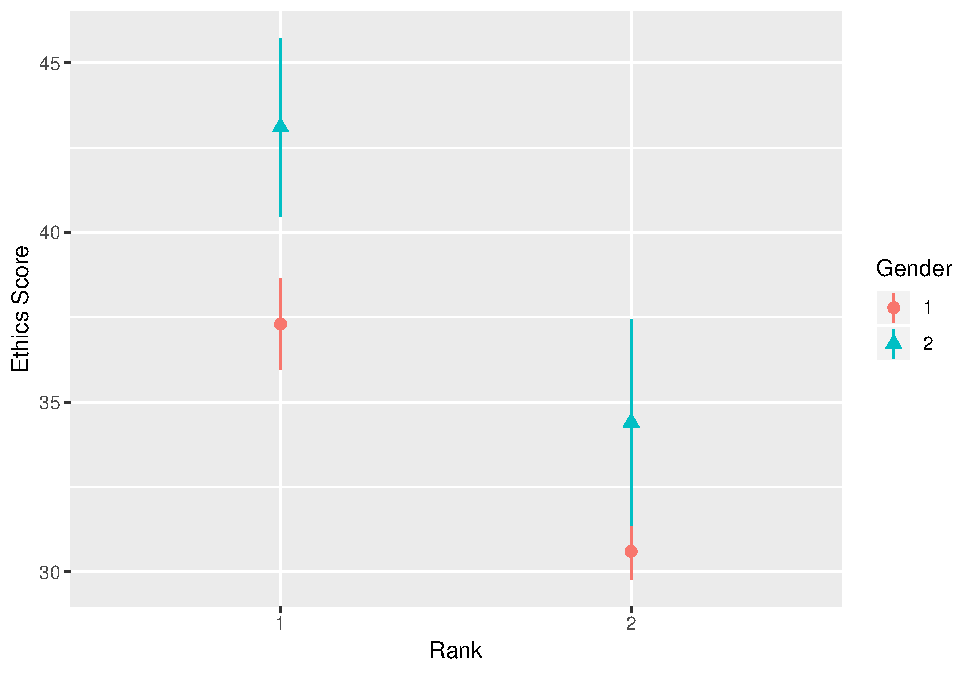
\includegraphics[width=0.3\linewidth]{lab7_stat565_files/figure-latex/unnamed-chunk-3-1}

\begin{enumerate}
\def\labelenumi{(\alph{enumi})}
\setcounter{enumi}{1}
\tightlist
\item
  \textcolor[rgb]{0.5,0.5,0.5}{Obtain the numerical summary for each treatment combination and factor levels separately. Report them here in a tabular form}
\end{enumerate}

\begin{longtable}[]{@{}cccccccccc@{}}
\toprule
\begin{minipage}[b]{0.08\columnwidth}\centering
Gender\strut
\end{minipage} & \begin{minipage}[b]{0.06\columnwidth}\centering
min\strut
\end{minipage} & \begin{minipage}[b]{0.07\columnwidth}\centering
Q1\strut
\end{minipage} & \begin{minipage}[b]{0.08\columnwidth}\centering
median\strut
\end{minipage} & \begin{minipage}[b]{0.07\columnwidth}\centering
Q3\strut
\end{minipage} & \begin{minipage}[b]{0.07\columnwidth}\centering
max\strut
\end{minipage} & \begin{minipage}[b]{0.07\columnwidth}\centering
mean\strut
\end{minipage} & \begin{minipage}[b]{0.07\columnwidth}\centering
sd\strut
\end{minipage} & \begin{minipage}[b]{0.05\columnwidth}\centering
n\strut
\end{minipage} & \begin{minipage}[b]{0.09\columnwidth}\centering
missing\strut
\end{minipage}\tabularnewline
\midrule
\endhead
\begin{minipage}[t]{0.08\columnwidth}\centering
1\strut
\end{minipage} & \begin{minipage}[t]{0.06\columnwidth}\centering
2.42\strut
\end{minipage} & \begin{minipage}[t]{0.07\columnwidth}\centering
25.04\strut
\end{minipage} & \begin{minipage}[t]{0.08\columnwidth}\centering
31.92\strut
\end{minipage} & \begin{minipage}[t]{0.07\columnwidth}\centering
40.11\strut
\end{minipage} & \begin{minipage}[t]{0.07\columnwidth}\centering
63.03\strut
\end{minipage} & \begin{minipage}[t]{0.07\columnwidth}\centering
32.51\strut
\end{minipage} & \begin{minipage}[t]{0.07\columnwidth}\centering
11.6\strut
\end{minipage} & \begin{minipage}[t]{0.05\columnwidth}\centering
252\strut
\end{minipage} & \begin{minipage}[t]{0.09\columnwidth}\centering
0\strut
\end{minipage}\tabularnewline
\begin{minipage}[t]{0.08\columnwidth}\centering
2\strut
\end{minipage} & \begin{minipage}[t]{0.06\columnwidth}\centering
5.65\strut
\end{minipage} & \begin{minipage}[t]{0.07\columnwidth}\centering
27.73\strut
\end{minipage} & \begin{minipage}[t]{0.08\columnwidth}\centering
37.57\strut
\end{minipage} & \begin{minipage}[t]{0.07\columnwidth}\centering
49.06\strut
\end{minipage} & \begin{minipage}[t]{0.07\columnwidth}\centering
65.22\strut
\end{minipage} & \begin{minipage}[t]{0.07\columnwidth}\centering
37.18\strut
\end{minipage} & \begin{minipage}[t]{0.07\columnwidth}\centering
15.72\strut
\end{minipage} & \begin{minipage}[t]{0.05\columnwidth}\centering
47\strut
\end{minipage} & \begin{minipage}[t]{0.09\columnwidth}\centering
0\strut
\end{minipage}\tabularnewline
\bottomrule
\end{longtable}

\begin{longtable}[]{@{}cccccccccc@{}}
\toprule
\begin{minipage}[b]{0.06\columnwidth}\centering
Rank\strut
\end{minipage} & \begin{minipage}[b]{0.07\columnwidth}\centering
min\strut
\end{minipage} & \begin{minipage}[b]{0.07\columnwidth}\centering
Q1\strut
\end{minipage} & \begin{minipage}[b]{0.08\columnwidth}\centering
median\strut
\end{minipage} & \begin{minipage}[b]{0.07\columnwidth}\centering
Q3\strut
\end{minipage} & \begin{minipage}[b]{0.07\columnwidth}\centering
max\strut
\end{minipage} & \begin{minipage}[b]{0.07\columnwidth}\centering
mean\strut
\end{minipage} & \begin{minipage}[b]{0.07\columnwidth}\centering
sd\strut
\end{minipage} & \begin{minipage}[b]{0.06\columnwidth}\centering
n\strut
\end{minipage} & \begin{minipage}[b]{0.09\columnwidth}\centering
missing\strut
\end{minipage}\tabularnewline
\midrule
\endhead
\begin{minipage}[t]{0.06\columnwidth}\centering
1\strut
\end{minipage} & \begin{minipage}[t]{0.07\columnwidth}\centering
11.91\strut
\end{minipage} & \begin{minipage}[t]{0.07\columnwidth}\centering
30.38\strut
\end{minipage} & \begin{minipage}[t]{0.08\columnwidth}\centering
37.19\strut
\end{minipage} & \begin{minipage}[t]{0.07\columnwidth}\centering
46.62\strut
\end{minipage} & \begin{minipage}[t]{0.07\columnwidth}\centering
62.1\strut
\end{minipage} & \begin{minipage}[t]{0.07\columnwidth}\centering
38.3\strut
\end{minipage} & \begin{minipage}[t]{0.07\columnwidth}\centering
11.34\strut
\end{minipage} & \begin{minipage}[t]{0.06\columnwidth}\centering
87\strut
\end{minipage} & \begin{minipage}[t]{0.09\columnwidth}\centering
0\strut
\end{minipage}\tabularnewline
\begin{minipage}[t]{0.06\columnwidth}\centering
2\strut
\end{minipage} & \begin{minipage}[t]{0.07\columnwidth}\centering
2.42\strut
\end{minipage} & \begin{minipage}[t]{0.07\columnwidth}\centering
23.44\strut
\end{minipage} & \begin{minipage}[t]{0.08\columnwidth}\centering
30.25\strut
\end{minipage} & \begin{minipage}[t]{0.07\columnwidth}\centering
39.37\strut
\end{minipage} & \begin{minipage}[t]{0.07\columnwidth}\centering
65.22\strut
\end{minipage} & \begin{minipage}[t]{0.07\columnwidth}\centering
31.17\strut
\end{minipage} & \begin{minipage}[t]{0.07\columnwidth}\centering
12.29\strut
\end{minipage} & \begin{minipage}[t]{0.06\columnwidth}\centering
212\strut
\end{minipage} & \begin{minipage}[t]{0.09\columnwidth}\centering
0\strut
\end{minipage}\tabularnewline
\bottomrule
\end{longtable}

\begin{longtable}[]{@{}cccccccccc@{}}
\toprule
\begin{minipage}[b]{0.12\columnwidth}\centering
Gender.Rank\strut
\end{minipage} & \begin{minipage}[b]{0.07\columnwidth}\centering
min\strut
\end{minipage} & \begin{minipage}[b]{0.07\columnwidth}\centering
Q1\strut
\end{minipage} & \begin{minipage}[b]{0.08\columnwidth}\centering
median\strut
\end{minipage} & \begin{minipage}[b]{0.07\columnwidth}\centering
Q3\strut
\end{minipage} & \begin{minipage}[b]{0.07\columnwidth}\centering
max\strut
\end{minipage} & \begin{minipage}[b]{0.06\columnwidth}\centering
mean\strut
\end{minipage} & \begin{minipage}[b]{0.07\columnwidth}\centering
sd\strut
\end{minipage} & \begin{minipage}[b]{0.05\columnwidth}\centering
n\strut
\end{minipage} & \begin{minipage}[b]{0.09\columnwidth}\centering
missing\strut
\end{minipage}\tabularnewline
\midrule
\endhead
\begin{minipage}[t]{0.12\columnwidth}\centering
1.1\strut
\end{minipage} & \begin{minipage}[t]{0.07\columnwidth}\centering
11.91\strut
\end{minipage} & \begin{minipage}[t]{0.07\columnwidth}\centering
30\strut
\end{minipage} & \begin{minipage}[t]{0.08\columnwidth}\centering
35.9\strut
\end{minipage} & \begin{minipage}[t]{0.07\columnwidth}\centering
45.22\strut
\end{minipage} & \begin{minipage}[t]{0.07\columnwidth}\centering
62.1\strut
\end{minipage} & \begin{minipage}[t]{0.06\columnwidth}\centering
37.3\strut
\end{minipage} & \begin{minipage}[t]{0.07\columnwidth}\centering
11.38\strut
\end{minipage} & \begin{minipage}[t]{0.05\columnwidth}\centering
72\strut
\end{minipage} & \begin{minipage}[t]{0.09\columnwidth}\centering
0\strut
\end{minipage}\tabularnewline
\begin{minipage}[t]{0.12\columnwidth}\centering
2.1\strut
\end{minipage} & \begin{minipage}[t]{0.07\columnwidth}\centering
27.65\strut
\end{minipage} & \begin{minipage}[t]{0.07\columnwidth}\centering
36.12\strut
\end{minipage} & \begin{minipage}[t]{0.08\columnwidth}\centering
44.74\strut
\end{minipage} & \begin{minipage}[t]{0.07\columnwidth}\centering
51\strut
\end{minipage} & \begin{minipage}[t]{0.07\columnwidth}\centering
60.11\strut
\end{minipage} & \begin{minipage}[t]{0.06\columnwidth}\centering
43.1\strut
\end{minipage} & \begin{minipage}[t]{0.07\columnwidth}\centering
10.14\strut
\end{minipage} & \begin{minipage}[t]{0.05\columnwidth}\centering
15\strut
\end{minipage} & \begin{minipage}[t]{0.09\columnwidth}\centering
0\strut
\end{minipage}\tabularnewline
\begin{minipage}[t]{0.12\columnwidth}\centering
1.2\strut
\end{minipage} & \begin{minipage}[t]{0.07\columnwidth}\centering
2.42\strut
\end{minipage} & \begin{minipage}[t]{0.07\columnwidth}\centering
23.65\strut
\end{minipage} & \begin{minipage}[t]{0.08\columnwidth}\centering
29.78\strut
\end{minipage} & \begin{minipage}[t]{0.07\columnwidth}\centering
38.39\strut
\end{minipage} & \begin{minipage}[t]{0.07\columnwidth}\centering
63.03\strut
\end{minipage} & \begin{minipage}[t]{0.06\columnwidth}\centering
30.6\strut
\end{minipage} & \begin{minipage}[t]{0.07\columnwidth}\centering
11.16\strut
\end{minipage} & \begin{minipage}[t]{0.05\columnwidth}\centering
180\strut
\end{minipage} & \begin{minipage}[t]{0.09\columnwidth}\centering
0\strut
\end{minipage}\tabularnewline
\begin{minipage}[t]{0.12\columnwidth}\centering
2.2\strut
\end{minipage} & \begin{minipage}[t]{0.07\columnwidth}\centering
5.65\strut
\end{minipage} & \begin{minipage}[t]{0.07\columnwidth}\centering
21.14\strut
\end{minipage} & \begin{minipage}[t]{0.08\columnwidth}\centering
30.75\strut
\end{minipage} & \begin{minipage}[t]{0.07\columnwidth}\centering
44.64\strut
\end{minipage} & \begin{minipage}[t]{0.07\columnwidth}\centering
65.22\strut
\end{minipage} & \begin{minipage}[t]{0.06\columnwidth}\centering
34.4\strut
\end{minipage} & \begin{minipage}[t]{0.07\columnwidth}\centering
17.19\strut
\end{minipage} & \begin{minipage}[t]{0.05\columnwidth}\centering
32\strut
\end{minipage} & \begin{minipage}[t]{0.09\columnwidth}\centering
0\strut
\end{minipage}\tabularnewline
\bottomrule
\end{longtable}

\begin{enumerate}
\def\labelenumi{(\alph{enumi})}
\setcounter{enumi}{2}
\tightlist
\item
  \textcolor[rgb]{0.5,0.5,0.5}{Fit the two-factor factorial model and report the complete ANOVA table here. Do not report code here. The complete ANOVA table should have a row for each of the following: main effects of each treatment, two-factor interaction effects, error and total.Report the adjusted (Type III) SS for each effect because of unbalanced design. Note that, adjusted SS and SSE do not add up to SSTotal}
\end{enumerate}

\begin{longtable}[]{@{}cllccc@{}}
\toprule
\begin{minipage}[b]{0.19\columnwidth}\centering
~\strut
\end{minipage} & \begin{minipage}[b]{0.07\columnwidth}\raggedright
Df\strut
\end{minipage} & \begin{minipage}[b]{0.13\columnwidth}\raggedright
Sum Sq\strut
\end{minipage} & \begin{minipage}[b]{0.12\columnwidth}\centering
Mean Sq\strut
\end{minipage} & \begin{minipage}[b]{0.12\columnwidth}\centering
F value\strut
\end{minipage} & \begin{minipage}[b]{0.14\columnwidth}\centering
Pr(\textgreater{}F)\strut
\end{minipage}\tabularnewline
\midrule
\endhead
\begin{minipage}[t]{0.19\columnwidth}\centering
\textbf{g}\strut
\end{minipage} & \begin{minipage}[t]{0.07\columnwidth}\raggedright
1\strut
\end{minipage} & \begin{minipage}[t]{0.13\columnwidth}\raggedright
860.9\strut
\end{minipage} & \begin{minipage}[t]{0.12\columnwidth}\centering
860.9\strut
\end{minipage} & \begin{minipage}[t]{0.12\columnwidth}\centering
6.034\strut
\end{minipage} & \begin{minipage}[t]{0.14\columnwidth}\centering
0.01461\strut
\end{minipage}\tabularnewline
\begin{minipage}[t]{0.19\columnwidth}\centering
\textbf{r}\strut
\end{minipage} & \begin{minipage}[t]{0.07\columnwidth}\raggedright
1\strut
\end{minipage} & \begin{minipage}[t]{0.13\columnwidth}\raggedright
3048\strut
\end{minipage} & \begin{minipage}[t]{0.12\columnwidth}\centering
3048\strut
\end{minipage} & \begin{minipage}[t]{0.12\columnwidth}\centering
21.36\strut
\end{minipage} & \begin{minipage}[t]{0.14\columnwidth}\centering
5.693e-06\strut
\end{minipage}\tabularnewline
\begin{minipage}[t]{0.19\columnwidth}\centering
\textbf{g:r}\strut
\end{minipage} & \begin{minipage}[t]{0.07\columnwidth}\raggedright
1\strut
\end{minipage} & \begin{minipage}[t]{0.13\columnwidth}\raggedright
34.1\strut
\end{minipage} & \begin{minipage}[t]{0.12\columnwidth}\centering
34.1\strut
\end{minipage} & \begin{minipage}[t]{0.12\columnwidth}\centering
0.239\strut
\end{minipage} & \begin{minipage}[t]{0.14\columnwidth}\centering
0.6253\strut
\end{minipage}\tabularnewline
\begin{minipage}[t]{0.19\columnwidth}\centering
\textbf{Residuals}\strut
\end{minipage} & \begin{minipage}[t]{0.07\columnwidth}\raggedright
295\strut
\end{minipage} & \begin{minipage}[t]{0.13\columnwidth}\raggedright
42087\strut
\end{minipage} & \begin{minipage}[t]{0.12\columnwidth}\centering
142.7\strut
\end{minipage} & \begin{minipage}[t]{0.12\columnwidth}\centering
NA\strut
\end{minipage} & \begin{minipage}[t]{0.14\columnwidth}\centering
NA\strut
\end{minipage}\tabularnewline
\begin{minipage}[t]{0.19\columnwidth}\centering
\textbf{Total}\strut
\end{minipage} & \begin{minipage}[t]{0.07\columnwidth}\raggedright
298\strut
\end{minipage} & \begin{minipage}[t]{0.13\columnwidth}\raggedright
46030.1\strut
\end{minipage} & \begin{minipage}[t]{0.12\columnwidth}\centering
154.46\strut
\end{minipage} & \begin{minipage}[t]{0.12\columnwidth}\centering
NA\strut
\end{minipage} & \begin{minipage}[t]{0.14\columnwidth}\centering
NA\strut
\end{minipage}\tabularnewline
\bottomrule
\end{longtable}

\begin{enumerate}
\def\labelenumi{(\alph{enumi})}
\setcounter{enumi}{3}
\tightlist
\item
  \textcolor[rgb]{0.5,0.5,0.5}{Based on the ANOVA table write your conclusion appropriately. Perform all the necessary tests and report the conclusion along with the p-value. (no need to do pairwise comparison to save the time)}
\end{enumerate}

The line plot shows that not all lines are parallel. Difference in y
between methods is not same for different varieties. There could be an
interaction effect.

According to ANOVA table, there is a significant interaction effect from
methods and varieties on the y at 5\% significance level
(P-value=0.02409). That means, effect of method and effect of methods
and varieties on y is not independent. Therefore, examie the simple
effects.

\begin{enumerate}
\def\labelenumi{(\alph{enumi})}
\setcounter{enumi}{4}
\tightlist
\item
  \textcolor[rgb]{0.5,0.5,0.5}{Report the code here without output.}
\end{enumerate}

\begin{Shaded}
\begin{Highlighting}[]
\KeywordTok{pander}\NormalTok{(}\KeywordTok{summary}\NormalTok{(model_ethics))}
\KeywordTok{sum}\NormalTok{((table_ethics}\OperatorTok{$}\NormalTok{Score }\OperatorTok{-}\StringTok{ }\KeywordTok{mean}\NormalTok{(table_ethics}\OperatorTok{$}\NormalTok{Score))}\OperatorTok{^}\DecValTok{2}\NormalTok{)}
\KeywordTok{Anova}\NormalTok{(model_ethics, }\DataTypeTok{type =} \StringTok{"III"}\NormalTok{)}
\end{Highlighting}
\end{Shaded}

\hypertarget{problem-2-3-factor-factorial-non-significant-interaction}{%
\section{Problem 2: 3-Factor Factorial (Non-significant
interaction)}\label{problem-2-3-factor-factorial-non-significant-interaction}}

\textcolor[rgb]{0.5,0.5,0.5}{Results from 3-Factor ANOVA to investigate effects of poker skill (average/expert), poker hand (bad/neutral/good), and bet limit (fixed/none) on winnings. There were 25 individuals in each of 12 combinations (each individual in only one treatment).Use a=0.05}

\textcolor[rgb]{0.5,0.5,0.5}{Variables/Columns:
Skill: 1=Expert, 2=Average; Hand:1=Bad, 2=Neutral, 3=Good; Limit: 1=Fixed, 2=None; Final Cash Balance (euros)}

\begin{enumerate}
\def\labelenumi{(\alph{enumi})}
\tightlist
\item
  \textcolor[rgb]{0.5,0.5,0.5}{Plot the data and report the plot here (A plot with data and means of treatment combinations). Do not report code here.}
\end{enumerate}

\begin{verbatim}
## 'data.frame':    300 obs. of  7 variables:
##  $ skill: int  1 1 1 1 1 1 1 1 1 1 ...
##  $ hand : int  1 1 1 1 1 1 1 1 1 1 ...
##  $ limit: int  1 1 1 1 1 1 1 1 1 1 ...
##  $ cash : num  4 5.55 9.45 7.19 5.71 5.32 8.52 4.06 4.97 6.18 ...
##  $ s    : Factor w/ 2 levels "Exp","Nov": 1 1 1 1 1 1 1 1 1 1 ...
##  $ h    : Factor w/ 3 levels "Bad","Neu","Goo": 1 1 1 1 1 1 1 1 1 1 ...
##  $ l    : Factor w/ 2 levels "Fix","Non": 1 1 1 1 1 1 1 1 1 1 ...
\end{verbatim}

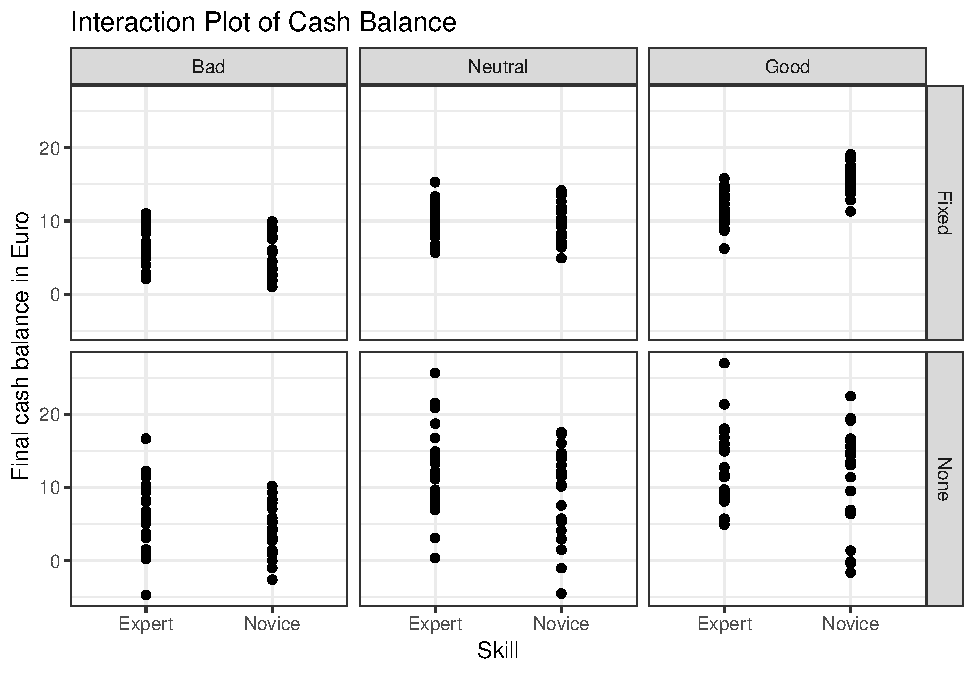
\includegraphics[width=0.3\linewidth]{lab7_stat565_files/figure-latex/unnamed-chunk-8-1}
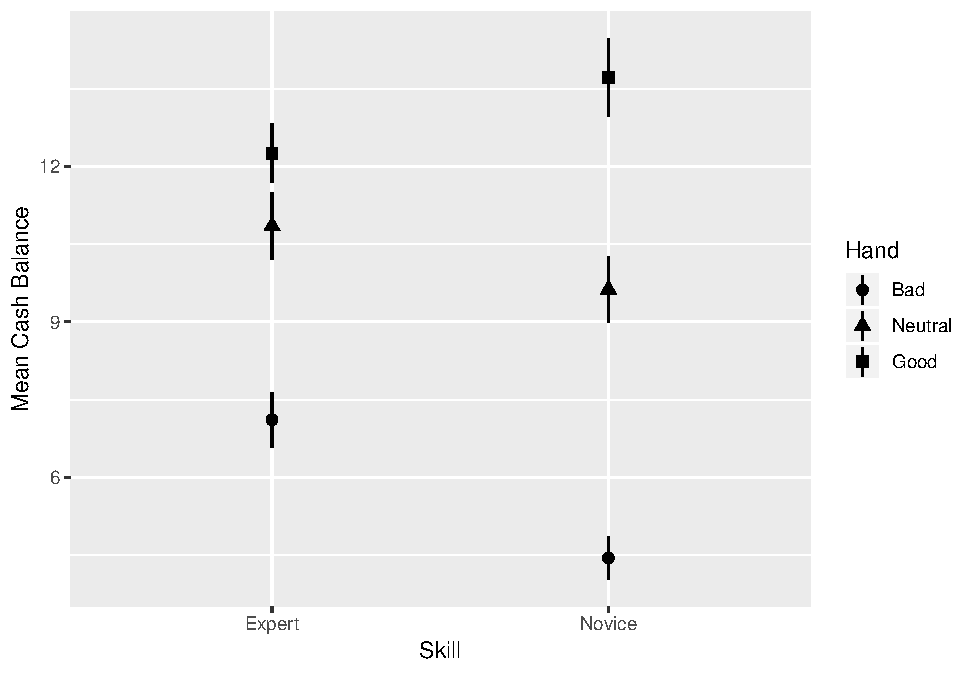
\includegraphics[width=0.3\linewidth]{lab7_stat565_files/figure-latex/unnamed-chunk-8-2}

\begin{enumerate}
\def\labelenumi{(\alph{enumi})}
\setcounter{enumi}{1}
\tightlist
\item
  \textcolor[rgb]{0.5,0.5,0.5}{Obtain the numerical summary for each treatment combination and factor levels separately. Report them here in a tabular form}
\end{enumerate}

\begin{longtable}[]{@{}cccccccccc@{}}
\toprule
\begin{minipage}[b]{0.06\columnwidth}\centering
s\strut
\end{minipage} & \begin{minipage}[b]{0.07\columnwidth}\centering
min\strut
\end{minipage} & \begin{minipage}[b]{0.07\columnwidth}\centering
Q1\strut
\end{minipage} & \begin{minipage}[b]{0.08\columnwidth}\centering
median\strut
\end{minipage} & \begin{minipage}[b]{0.07\columnwidth}\centering
Q3\strut
\end{minipage} & \begin{minipage}[b]{0.07\columnwidth}\centering
max\strut
\end{minipage} & \begin{minipage}[b]{0.07\columnwidth}\centering
mean\strut
\end{minipage} & \begin{minipage}[b]{0.07\columnwidth}\centering
sd\strut
\end{minipage} & \begin{minipage}[b]{0.06\columnwidth}\centering
n\strut
\end{minipage} & \begin{minipage}[b]{0.09\columnwidth}\centering
missing\strut
\end{minipage}\tabularnewline
\midrule
\endhead
\begin{minipage}[t]{0.06\columnwidth}\centering
Exp\strut
\end{minipage} & \begin{minipage}[t]{0.07\columnwidth}\centering
-4.68\strut
\end{minipage} & \begin{minipage}[t]{0.07\columnwidth}\centering
7.145\strut
\end{minipage} & \begin{minipage}[t]{0.08\columnwidth}\centering
9.59\strut
\end{minipage} & \begin{minipage}[t]{0.07\columnwidth}\centering
12.35\strut
\end{minipage} & \begin{minipage}[t]{0.07\columnwidth}\centering
26.99\strut
\end{minipage} & \begin{minipage}[t]{0.07\columnwidth}\centering
10.07\strut
\end{minipage} & \begin{minipage}[t]{0.07\columnwidth}\centering
4.64\strut
\end{minipage} & \begin{minipage}[t]{0.06\columnwidth}\centering
150\strut
\end{minipage} & \begin{minipage}[t]{0.09\columnwidth}\centering
0\strut
\end{minipage}\tabularnewline
\begin{minipage}[t]{0.06\columnwidth}\centering
Nov\strut
\end{minipage} & \begin{minipage}[t]{0.07\columnwidth}\centering
-4.47\strut
\end{minipage} & \begin{minipage}[t]{0.07\columnwidth}\centering
4.4\strut
\end{minipage} & \begin{minipage}[t]{0.08\columnwidth}\centering
9.415\strut
\end{minipage} & \begin{minipage}[t]{0.07\columnwidth}\centering
14.16\strut
\end{minipage} & \begin{minipage}[t]{0.07\columnwidth}\centering
22.48\strut
\end{minipage} & \begin{minipage}[t]{0.07\columnwidth}\centering
9.262\strut
\end{minipage} & \begin{minipage}[t]{0.07\columnwidth}\centering
5.755\strut
\end{minipage} & \begin{minipage}[t]{0.06\columnwidth}\centering
150\strut
\end{minipage} & \begin{minipage}[t]{0.09\columnwidth}\centering
0\strut
\end{minipage}\tabularnewline
\bottomrule
\end{longtable}

\begin{longtable}[]{@{}cccccccccc@{}}
\toprule
\begin{minipage}[b]{0.06\columnwidth}\centering
h\strut
\end{minipage} & \begin{minipage}[b]{0.07\columnwidth}\centering
min\strut
\end{minipage} & \begin{minipage}[b]{0.07\columnwidth}\centering
Q1\strut
\end{minipage} & \begin{minipage}[b]{0.08\columnwidth}\centering
median\strut
\end{minipage} & \begin{minipage}[b]{0.07\columnwidth}\centering
Q3\strut
\end{minipage} & \begin{minipage}[b]{0.07\columnwidth}\centering
max\strut
\end{minipage} & \begin{minipage}[b]{0.07\columnwidth}\centering
mean\strut
\end{minipage} & \begin{minipage}[b]{0.07\columnwidth}\centering
sd\strut
\end{minipage} & \begin{minipage}[b]{0.06\columnwidth}\centering
n\strut
\end{minipage} & \begin{minipage}[b]{0.09\columnwidth}\centering
missing\strut
\end{minipage}\tabularnewline
\midrule
\endhead
\begin{minipage}[t]{0.06\columnwidth}\centering
Bad\strut
\end{minipage} & \begin{minipage}[t]{0.07\columnwidth}\centering
-4.68\strut
\end{minipage} & \begin{minipage}[t]{0.07\columnwidth}\centering
3.4\strut
\end{minipage} & \begin{minipage}[t]{0.08\columnwidth}\centering
5.7\strut
\end{minipage} & \begin{minipage}[t]{0.07\columnwidth}\centering
8.41\strut
\end{minipage} & \begin{minipage}[t]{0.07\columnwidth}\centering
16.68\strut
\end{minipage} & \begin{minipage}[t]{0.07\columnwidth}\centering
5.777\strut
\end{minipage} & \begin{minipage}[t]{0.07\columnwidth}\centering
3.618\strut
\end{minipage} & \begin{minipage}[t]{0.06\columnwidth}\centering
100\strut
\end{minipage} & \begin{minipage}[t]{0.09\columnwidth}\centering
0\strut
\end{minipage}\tabularnewline
\begin{minipage}[t]{0.06\columnwidth}\centering
Neu\strut
\end{minipage} & \begin{minipage}[t]{0.07\columnwidth}\centering
-4.47\strut
\end{minipage} & \begin{minipage}[t]{0.07\columnwidth}\centering
7.827\strut
\end{minipage} & \begin{minipage}[t]{0.08\columnwidth}\centering
10.16\strut
\end{minipage} & \begin{minipage}[t]{0.07\columnwidth}\centering
12.39\strut
\end{minipage} & \begin{minipage}[t]{0.07\columnwidth}\centering
25.63\strut
\end{minipage} & \begin{minipage}[t]{0.07\columnwidth}\centering
10.24\strut
\end{minipage} & \begin{minipage}[t]{0.07\columnwidth}\centering
4.501\strut
\end{minipage} & \begin{minipage}[t]{0.06\columnwidth}\centering
100\strut
\end{minipage} & \begin{minipage}[t]{0.09\columnwidth}\centering
0\strut
\end{minipage}\tabularnewline
\begin{minipage}[t]{0.06\columnwidth}\centering
Goo\strut
\end{minipage} & \begin{minipage}[t]{0.07\columnwidth}\centering
-1.61\strut
\end{minipage} & \begin{minipage}[t]{0.07\columnwidth}\centering
9.713\strut
\end{minipage} & \begin{minipage}[t]{0.08\columnwidth}\centering
13.96\strut
\end{minipage} & \begin{minipage}[t]{0.07\columnwidth}\centering
15.98\strut
\end{minipage} & \begin{minipage}[t]{0.07\columnwidth}\centering
26.99\strut
\end{minipage} & \begin{minipage}[t]{0.07\columnwidth}\centering
12.98\strut
\end{minipage} & \begin{minipage}[t]{0.07\columnwidth}\centering
4.762\strut
\end{minipage} & \begin{minipage}[t]{0.06\columnwidth}\centering
100\strut
\end{minipage} & \begin{minipage}[t]{0.09\columnwidth}\centering
0\strut
\end{minipage}\tabularnewline
\bottomrule
\end{longtable}

\begin{longtable}[]{@{}cccccccccc@{}}
\toprule
\begin{minipage}[b]{0.12\columnwidth}\centering
s.h.l\strut
\end{minipage} & \begin{minipage}[b]{0.07\columnwidth}\centering
min\strut
\end{minipage} & \begin{minipage}[b]{0.07\columnwidth}\centering
Q1\strut
\end{minipage} & \begin{minipage}[b]{0.08\columnwidth}\centering
median\strut
\end{minipage} & \begin{minipage}[b]{0.07\columnwidth}\centering
Q3\strut
\end{minipage} & \begin{minipage}[b]{0.07\columnwidth}\centering
max\strut
\end{minipage} & \begin{minipage}[b]{0.07\columnwidth}\centering
mean\strut
\end{minipage} & \begin{minipage}[b]{0.07\columnwidth}\centering
sd\strut
\end{minipage} & \begin{minipage}[b]{0.04\columnwidth}\centering
n\strut
\end{minipage} & \begin{minipage}[b]{0.09\columnwidth}\centering
missing\strut
\end{minipage}\tabularnewline
\midrule
\endhead
\begin{minipage}[t]{0.12\columnwidth}\centering
Exp.Bad.Fix\strut
\end{minipage} & \begin{minipage}[t]{0.07\columnwidth}\centering
2.07\strut
\end{minipage} & \begin{minipage}[t]{0.07\columnwidth}\centering
5.55\strut
\end{minipage} & \begin{minipage}[t]{0.08\columnwidth}\centering
7.19\strut
\end{minipage} & \begin{minipage}[t]{0.07\columnwidth}\centering
9.45\strut
\end{minipage} & \begin{minipage}[t]{0.07\columnwidth}\centering
11.04\strut
\end{minipage} & \begin{minipage}[t]{0.07\columnwidth}\centering
7.329\strut
\end{minipage} & \begin{minipage}[t]{0.07\columnwidth}\centering
2.56\strut
\end{minipage} & \begin{minipage}[t]{0.04\columnwidth}\centering
25\strut
\end{minipage} & \begin{minipage}[t]{0.09\columnwidth}\centering
0\strut
\end{minipage}\tabularnewline
\begin{minipage}[t]{0.12\columnwidth}\centering
Nov.Bad.Fix\strut
\end{minipage} & \begin{minipage}[t]{0.07\columnwidth}\centering
1.02\strut
\end{minipage} & \begin{minipage}[t]{0.07\columnwidth}\centering
3.43\strut
\end{minipage} & \begin{minipage}[t]{0.08\columnwidth}\centering
4.39\strut
\end{minipage} & \begin{minipage}[t]{0.07\columnwidth}\centering
7.53\strut
\end{minipage} & \begin{minipage}[t]{0.07\columnwidth}\centering
9.94\strut
\end{minipage} & \begin{minipage}[t]{0.07\columnwidth}\centering
5.05\strut
\end{minipage} & \begin{minipage}[t]{0.07\columnwidth}\centering
2.55\strut
\end{minipage} & \begin{minipage}[t]{0.04\columnwidth}\centering
25\strut
\end{minipage} & \begin{minipage}[t]{0.09\columnwidth}\centering
0\strut
\end{minipage}\tabularnewline
\begin{minipage}[t]{0.12\columnwidth}\centering
Exp.Neu.Fix\strut
\end{minipage} & \begin{minipage}[t]{0.07\columnwidth}\centering
5.68\strut
\end{minipage} & \begin{minipage}[t]{0.07\columnwidth}\centering
8.33\strut
\end{minipage} & \begin{minipage}[t]{0.08\columnwidth}\centering
9.51\strut
\end{minipage} & \begin{minipage}[t]{0.07\columnwidth}\centering
11.56\strut
\end{minipage} & \begin{minipage}[t]{0.07\columnwidth}\centering
15.3\strut
\end{minipage} & \begin{minipage}[t]{0.07\columnwidth}\centering
9.85\strut
\end{minipage} & \begin{minipage}[t]{0.07\columnwidth}\centering
2.52\strut
\end{minipage} & \begin{minipage}[t]{0.04\columnwidth}\centering
25\strut
\end{minipage} & \begin{minipage}[t]{0.09\columnwidth}\centering
0\strut
\end{minipage}\tabularnewline
\begin{minipage}[t]{0.12\columnwidth}\centering
Nov.Neu.Fix\strut
\end{minipage} & \begin{minipage}[t]{0.07\columnwidth}\centering
4.93\strut
\end{minipage} & \begin{minipage}[t]{0.07\columnwidth}\centering
8.21\strut
\end{minipage} & \begin{minipage}[t]{0.08\columnwidth}\centering
9.62\strut
\end{minipage} & \begin{minipage}[t]{0.07\columnwidth}\centering
11.63\strut
\end{minipage} & \begin{minipage}[t]{0.07\columnwidth}\centering
14.18\strut
\end{minipage} & \begin{minipage}[t]{0.07\columnwidth}\centering
9.8\strut
\end{minipage} & \begin{minipage}[t]{0.07\columnwidth}\centering
2.42\strut
\end{minipage} & \begin{minipage}[t]{0.04\columnwidth}\centering
25\strut
\end{minipage} & \begin{minipage}[t]{0.09\columnwidth}\centering
0\strut
\end{minipage}\tabularnewline
\begin{minipage}[t]{0.12\columnwidth}\centering
Exp.Goo.Fix\strut
\end{minipage} & \begin{minipage}[t]{0.07\columnwidth}\centering
6.24\strut
\end{minipage} & \begin{minipage}[t]{0.07\columnwidth}\centering
10.56\strut
\end{minipage} & \begin{minipage}[t]{0.08\columnwidth}\centering
12.37\strut
\end{minipage} & \begin{minipage}[t]{0.07\columnwidth}\centering
14.12\strut
\end{minipage} & \begin{minipage}[t]{0.07\columnwidth}\centering
15.84\strut
\end{minipage} & \begin{minipage}[t]{0.07\columnwidth}\centering
12.12\strut
\end{minipage} & \begin{minipage}[t]{0.07\columnwidth}\centering
2.32\strut
\end{minipage} & \begin{minipage}[t]{0.04\columnwidth}\centering
25\strut
\end{minipage} & \begin{minipage}[t]{0.09\columnwidth}\centering
0\strut
\end{minipage}\tabularnewline
\begin{minipage}[t]{0.12\columnwidth}\centering
Nov.Goo.Fix\strut
\end{minipage} & \begin{minipage}[t]{0.07\columnwidth}\centering
11.31\strut
\end{minipage} & \begin{minipage}[t]{0.07\columnwidth}\centering
14.49\strut
\end{minipage} & \begin{minipage}[t]{0.08\columnwidth}\centering
16.09\strut
\end{minipage} & \begin{minipage}[t]{0.07\columnwidth}\centering
17.27\strut
\end{minipage} & \begin{minipage}[t]{0.07\columnwidth}\centering
19.11\strut
\end{minipage} & \begin{minipage}[t]{0.07\columnwidth}\centering
15.8\strut
\end{minipage} & \begin{minipage}[t]{0.07\columnwidth}\centering
1.94\strut
\end{minipage} & \begin{minipage}[t]{0.04\columnwidth}\centering
25\strut
\end{minipage} & \begin{minipage}[t]{0.09\columnwidth}\centering
0\strut
\end{minipage}\tabularnewline
\begin{minipage}[t]{0.12\columnwidth}\centering
Exp.Bad.Non\strut
\end{minipage} & \begin{minipage}[t]{0.07\columnwidth}\centering
-4.68\strut
\end{minipage} & \begin{minipage}[t]{0.07\columnwidth}\centering
3.82\strut
\end{minipage} & \begin{minipage}[t]{0.08\columnwidth}\centering
6.42\strut
\end{minipage} & \begin{minipage}[t]{0.07\columnwidth}\centering
10.34\strut
\end{minipage} & \begin{minipage}[t]{0.07\columnwidth}\centering
16.68\strut
\end{minipage} & \begin{minipage}[t]{0.07\columnwidth}\centering
6.889\strut
\end{minipage} & \begin{minipage}[t]{0.07\columnwidth}\centering
4.71\strut
\end{minipage} & \begin{minipage}[t]{0.04\columnwidth}\centering
25\strut
\end{minipage} & \begin{minipage}[t]{0.09\columnwidth}\centering
0\strut
\end{minipage}\tabularnewline
\begin{minipage}[t]{0.12\columnwidth}\centering
Nov.Bad.Non\strut
\end{minipage} & \begin{minipage}[t]{0.07\columnwidth}\centering
-2.57\strut
\end{minipage} & \begin{minipage}[t]{0.07\columnwidth}\centering
1.19\strut
\end{minipage} & \begin{minipage}[t]{0.08\columnwidth}\centering
4.02\strut
\end{minipage} & \begin{minipage}[t]{0.07\columnwidth}\centering
5.82\strut
\end{minipage} & \begin{minipage}[t]{0.07\columnwidth}\centering
10.19\strut
\end{minipage} & \begin{minipage}[t]{0.07\columnwidth}\centering
3.84\strut
\end{minipage} & \begin{minipage}[t]{0.07\columnwidth}\centering
3.24\strut
\end{minipage} & \begin{minipage}[t]{0.04\columnwidth}\centering
25\strut
\end{minipage} & \begin{minipage}[t]{0.09\columnwidth}\centering
0\strut
\end{minipage}\tabularnewline
\begin{minipage}[t]{0.12\columnwidth}\centering
Exp.Neu.Non\strut
\end{minipage} & \begin{minipage}[t]{0.07\columnwidth}\centering
0.39\strut
\end{minipage} & \begin{minipage}[t]{0.07\columnwidth}\centering
8.31\strut
\end{minipage} & \begin{minipage}[t]{0.08\columnwidth}\centering
11.14\strut
\end{minipage} & \begin{minipage}[t]{0.07\columnwidth}\centering
14.53\strut
\end{minipage} & \begin{minipage}[t]{0.07\columnwidth}\centering
25.63\strut
\end{minipage} & \begin{minipage}[t]{0.07\columnwidth}\centering
11.85\strut
\end{minipage} & \begin{minipage}[t]{0.07\columnwidth}\centering
5.771\strut
\end{minipage} & \begin{minipage}[t]{0.04\columnwidth}\centering
25\strut
\end{minipage} & \begin{minipage}[t]{0.09\columnwidth}\centering
0\strut
\end{minipage}\tabularnewline
\begin{minipage}[t]{0.12\columnwidth}\centering
Nov.Neu.Non\strut
\end{minipage} & \begin{minipage}[t]{0.07\columnwidth}\centering
-4.47\strut
\end{minipage} & \begin{minipage}[t]{0.07\columnwidth}\centering
5.32\strut
\end{minipage} & \begin{minipage}[t]{0.08\columnwidth}\centering
11.48\strut
\end{minipage} & \begin{minipage}[t]{0.07\columnwidth}\centering
13.93\strut
\end{minipage} & \begin{minipage}[t]{0.07\columnwidth}\centering
17.56\strut
\end{minipage} & \begin{minipage}[t]{0.07\columnwidth}\centering
9.45\strut
\end{minipage} & \begin{minipage}[t]{0.07\columnwidth}\centering
5.861\strut
\end{minipage} & \begin{minipage}[t]{0.04\columnwidth}\centering
25\strut
\end{minipage} & \begin{minipage}[t]{0.09\columnwidth}\centering
0\strut
\end{minipage}\tabularnewline
\begin{minipage}[t]{0.12\columnwidth}\centering
Exp.Goo.Non\strut
\end{minipage} & \begin{minipage}[t]{0.07\columnwidth}\centering
4.93\strut
\end{minipage} & \begin{minipage}[t]{0.07\columnwidth}\centering
8.76\strut
\end{minipage} & \begin{minipage}[t]{0.08\columnwidth}\centering
11.44\strut
\end{minipage} & \begin{minipage}[t]{0.07\columnwidth}\centering
15.33\strut
\end{minipage} & \begin{minipage}[t]{0.07\columnwidth}\centering
26.99\strut
\end{minipage} & \begin{minipage}[t]{0.07\columnwidth}\centering
12.39\strut
\end{minipage} & \begin{minipage}[t]{0.07\columnwidth}\centering
5.31\strut
\end{minipage} & \begin{minipage}[t]{0.04\columnwidth}\centering
25\strut
\end{minipage} & \begin{minipage}[t]{0.09\columnwidth}\centering
0\strut
\end{minipage}\tabularnewline
\begin{minipage}[t]{0.12\columnwidth}\centering
Nov.Goo.Non\strut
\end{minipage} & \begin{minipage}[t]{0.07\columnwidth}\centering
-1.61\strut
\end{minipage} & \begin{minipage}[t]{0.07\columnwidth}\centering
6.94\strut
\end{minipage} & \begin{minipage}[t]{0.08\columnwidth}\centering
13.55\strut
\end{minipage} & \begin{minipage}[t]{0.07\columnwidth}\centering
16.31\strut
\end{minipage} & \begin{minipage}[t]{0.07\columnwidth}\centering
22.48\strut
\end{minipage} & \begin{minipage}[t]{0.07\columnwidth}\centering
11.63\strut
\end{minipage} & \begin{minipage}[t]{0.07\columnwidth}\centering
6.7\strut
\end{minipage} & \begin{minipage}[t]{0.04\columnwidth}\centering
25\strut
\end{minipage} & \begin{minipage}[t]{0.09\columnwidth}\centering
0\strut
\end{minipage}\tabularnewline
\bottomrule
\end{longtable}

\begin{enumerate}
\def\labelenumi{(\alph{enumi})}
\setcounter{enumi}{2}
\tightlist
\item
  \textcolor[rgb]{0.5,0.5,0.5}{Fit the two-factor factorial model and report the complete ANOVA table here. Do not report code here. The complete ANOVA table should have a row for each of the following: main effects of each treatment, two-factor interaction effects, error and total.}
\end{enumerate}

\begin{longtable}[]{@{}cccccc@{}}
\toprule
\begin{minipage}[b]{0.19\columnwidth}\centering
~\strut
\end{minipage} & \begin{minipage}[b]{0.07\columnwidth}\centering
Df\strut
\end{minipage} & \begin{minipage}[b]{0.12\columnwidth}\centering
Sum Sq\strut
\end{minipage} & \begin{minipage}[b]{0.12\columnwidth}\centering
Mean Sq\strut
\end{minipage} & \begin{minipage}[b]{0.12\columnwidth}\centering
F value\strut
\end{minipage} & \begin{minipage}[b]{0.14\columnwidth}\centering
Pr(\textgreater{}F)\strut
\end{minipage}\tabularnewline
\midrule
\endhead
\begin{minipage}[t]{0.19\columnwidth}\centering
\textbf{s}\strut
\end{minipage} & \begin{minipage}[t]{0.07\columnwidth}\centering
1\strut
\end{minipage} & \begin{minipage}[t]{0.12\columnwidth}\centering
49.17\strut
\end{minipage} & \begin{minipage}[t]{0.12\columnwidth}\centering
49.17\strut
\end{minipage} & \begin{minipage}[t]{0.12\columnwidth}\centering
2.839\strut
\end{minipage} & \begin{minipage}[t]{0.14\columnwidth}\centering
0.09308\strut
\end{minipage}\tabularnewline
\begin{minipage}[t]{0.19\columnwidth}\centering
\textbf{h}\strut
\end{minipage} & \begin{minipage}[t]{0.07\columnwidth}\centering
2\strut
\end{minipage} & \begin{minipage}[t]{0.12\columnwidth}\centering
2647\strut
\end{minipage} & \begin{minipage}[t]{0.12\columnwidth}\centering
1323\strut
\end{minipage} & \begin{minipage}[t]{0.12\columnwidth}\centering
76.41\strut
\end{minipage} & \begin{minipage}[t]{0.14\columnwidth}\centering
2.389e-27\strut
\end{minipage}\tabularnewline
\begin{minipage}[t]{0.19\columnwidth}\centering
\textbf{l}\strut
\end{minipage} & \begin{minipage}[t]{0.07\columnwidth}\centering
1\strut
\end{minipage} & \begin{minipage}[t]{0.12\columnwidth}\centering
31.68\strut
\end{minipage} & \begin{minipage}[t]{0.12\columnwidth}\centering
31.68\strut
\end{minipage} & \begin{minipage}[t]{0.12\columnwidth}\centering
1.829\strut
\end{minipage} & \begin{minipage}[t]{0.14\columnwidth}\centering
0.1773\strut
\end{minipage}\tabularnewline
\begin{minipage}[t]{0.19\columnwidth}\centering
\textbf{s:h}\strut
\end{minipage} & \begin{minipage}[t]{0.07\columnwidth}\centering
2\strut
\end{minipage} & \begin{minipage}[t]{0.12\columnwidth}\centering
219\strut
\end{minipage} & \begin{minipage}[t]{0.12\columnwidth}\centering
109.5\strut
\end{minipage} & \begin{minipage}[t]{0.12\columnwidth}\centering
6.324\strut
\end{minipage} & \begin{minipage}[t]{0.14\columnwidth}\centering
0.002052\strut
\end{minipage}\tabularnewline
\begin{minipage}[t]{0.19\columnwidth}\centering
\textbf{s:l}\strut
\end{minipage} & \begin{minipage}[t]{0.07\columnwidth}\centering
1\strut
\end{minipage} & \begin{minipage}[t]{0.12\columnwidth}\centering
119.1\strut
\end{minipage} & \begin{minipage}[t]{0.12\columnwidth}\centering
119.1\strut
\end{minipage} & \begin{minipage}[t]{0.12\columnwidth}\centering
6.878\strut
\end{minipage} & \begin{minipage}[t]{0.14\columnwidth}\centering
0.009191\strut
\end{minipage}\tabularnewline
\begin{minipage}[t]{0.19\columnwidth}\centering
\textbf{h:l}\strut
\end{minipage} & \begin{minipage}[t]{0.07\columnwidth}\centering
2\strut
\end{minipage} & \begin{minipage}[t]{0.12\columnwidth}\centering
97.29\strut
\end{minipage} & \begin{minipage}[t]{0.12\columnwidth}\centering
48.64\strut
\end{minipage} & \begin{minipage}[t]{0.12\columnwidth}\centering
2.809\strut
\end{minipage} & \begin{minipage}[t]{0.14\columnwidth}\centering
0.06192\strut
\end{minipage}\tabularnewline
\begin{minipage}[t]{0.19\columnwidth}\centering
\textbf{s:h:l}\strut
\end{minipage} & \begin{minipage}[t]{0.07\columnwidth}\centering
2\strut
\end{minipage} & \begin{minipage}[t]{0.12\columnwidth}\centering
42.38\strut
\end{minipage} & \begin{minipage}[t]{0.12\columnwidth}\centering
21.19\strut
\end{minipage} & \begin{minipage}[t]{0.12\columnwidth}\centering
1.224\strut
\end{minipage} & \begin{minipage}[t]{0.14\columnwidth}\centering
0.2957\strut
\end{minipage}\tabularnewline
\begin{minipage}[t]{0.19\columnwidth}\centering
\textbf{Residuals}\strut
\end{minipage} & \begin{minipage}[t]{0.07\columnwidth}\centering
288\strut
\end{minipage} & \begin{minipage}[t]{0.12\columnwidth}\centering
4987\strut
\end{minipage} & \begin{minipage}[t]{0.12\columnwidth}\centering
17.32\strut
\end{minipage} & \begin{minipage}[t]{0.12\columnwidth}\centering
NA\strut
\end{minipage} & \begin{minipage}[t]{0.14\columnwidth}\centering
NA\strut
\end{minipage}\tabularnewline
\begin{minipage}[t]{0.19\columnwidth}\centering
\textbf{Total}\strut
\end{minipage} & \begin{minipage}[t]{0.07\columnwidth}\centering
299\strut
\end{minipage} & \begin{minipage}[t]{0.12\columnwidth}\centering
8192.67\strut
\end{minipage} & \begin{minipage}[t]{0.12\columnwidth}\centering
27.40\strut
\end{minipage} & \begin{minipage}[t]{0.12\columnwidth}\centering
NA\strut
\end{minipage} & \begin{minipage}[t]{0.14\columnwidth}\centering
NA\strut
\end{minipage}\tabularnewline
\bottomrule
\end{longtable}

\begin{enumerate}
\def\labelenumi{(\alph{enumi})}
\setcounter{enumi}{3}
\tightlist
\item
  \textcolor[rgb]{0.5,0.5,0.5}{Based on the ANOVA table write your conclusion appropriately. Perform all the necessary tests and report the conclusion along with the p-value.}
\end{enumerate}

The line plot shows that not all lines are parallel. Difference in y
between methods is not same for different varieties. There could be an
interaction effect.

According to ANOVA table, there is a significant interaction effect from
methods and varieties on the y at 5\% significance level
(P-value=0.02409). That means, effect of method and effect of methods
and varieties on y is not independent. Therefore, examie the simple
effects.

\begin{enumerate}
\def\labelenumi{(\alph{enumi})}
\setcounter{enumi}{4}
\item
  \textcolor[rgb]{0.5,0.5,0.5}{Suppose that we want to compare the average final cash balance between two types of Skill (Expert versus Average) when the type of Hand is 3 (Good) and Limit is 1 (Fixed). This is the simple effect contrast we learned in class. Test this contrast and report conclusion with p value.}
\item
  \textcolor[rgb]{0.5,0.5,0.5}{Report the code here without output.}
\end{enumerate}

\begin{Shaded}
\begin{Highlighting}[]
\CommentTok{# If the 3-factor interaction is significant, then test 2-factor interaction}
\CommentTok{# for each level of 3rd factor# To do all pairwise comparisons at each level}
\CommentTok{# of skill(s) factor # Load lsmeans or emmeans package #}
\KeywordTok{contrast}\NormalTok{(}\KeywordTok{lsmeans}\NormalTok{(model_poker, }\OperatorTok{~}\NormalTok{h }\OperatorTok{*}\StringTok{ }\NormalTok{l }\OperatorTok{|}\StringTok{ }\NormalTok{s), }\DataTypeTok{interaction =} \StringTok{"pairwise"}\NormalTok{)  }\CommentTok{# You may use and adjustment method as shown in the next contrast #}
\end{Highlighting}
\end{Shaded}

\begin{verbatim}
## s = Exp:
##  h_pairwise l_pairwise estimate   SE  df t.ratio p.value
##  Bad - Neu  Fix - Non     2.439 1.66 288  1.465  0.1440 
##  Bad - Goo  Fix - Non     0.712 1.66 288  0.428  0.6692 
##  Neu - Goo  Fix - Non    -1.727 1.66 288 -1.037  0.3004 
## 
## s = Nov:
##  h_pairwise l_pairwise estimate   SE  df t.ratio p.value
##  Bad - Neu  Fix - Non     0.861 1.66 288  0.517  0.6055 
##  Bad - Goo  Fix - Non    -2.959 1.66 288 -1.778  0.0765 
##  Neu - Goo  Fix - Non    -3.820 1.66 288 -2.295  0.0225
\end{verbatim}

\begin{Shaded}
\begin{Highlighting}[]
\CommentTok{# To do all pairwise comparisons at each level of hand (h) factor # Load}
\CommentTok{# lsmeans or emmeans package #}
\KeywordTok{contrast}\NormalTok{(}\KeywordTok{lsmeans}\NormalTok{(model_poker, }\OperatorTok{~}\NormalTok{s }\OperatorTok{*}\StringTok{ }\NormalTok{l }\OperatorTok{|}\StringTok{ }\NormalTok{h), }\DataTypeTok{interaction =} \StringTok{"pairwise"}\NormalTok{, }\DataTypeTok{adjust =} \StringTok{"bonferroni"}\NormalTok{)}
\end{Highlighting}
\end{Shaded}

\begin{verbatim}
## h = Bad:
##  s_pairwise l_pairwise estimate   SE  df t.ratio p.value
##  Exp - Nov  Fix - Non    -0.771 1.66 288 -0.463  0.6437 
## 
## h = Neu:
##  s_pairwise l_pairwise estimate   SE  df t.ratio p.value
##  Exp - Nov  Fix - Non    -2.349 1.66 288 -1.411  0.1593 
## 
## h = Goo:
##  s_pairwise l_pairwise estimate   SE  df t.ratio p.value
##  Exp - Nov  Fix - Non    -4.442 1.66 288 -2.668  0.0081
\end{verbatim}

\begin{Shaded}
\begin{Highlighting}[]
\CommentTok{# To write contrasts in terms of cell means # First, create a 3-factor}
\CommentTok{# interaction term of factors s, h and l # Then fit the model with that}
\CommentTok{# factor #}
\NormalTok{table_poker}\OperatorTok{$}\NormalTok{shl <-}\StringTok{ }\KeywordTok{interaction}\NormalTok{(table_poker}\OperatorTok{$}\NormalTok{s, table_poker}\OperatorTok{$}\NormalTok{h, table_poker}\OperatorTok{$}\NormalTok{l)}
\CommentTok{# Load lsmeans or emmeans package # Save the LSmeans for interaction terms}
\CommentTok{# of factors s, h and l #}

\CommentTok{# Before writing a contrast, check the order of terms in previous lsmf}
\CommentTok{# output # Then create a vector of contrast in terms of LSmeans of treatment}
\CommentTok{# combinations # Below is the contrast to test mean for two levels of skill}
\CommentTok{# factor (Expert versus Average) # when the type of Hand is 3 (Good) and}
\CommentTok{# Limit is 1 (Fixed) #}
\KeywordTok{summary}\NormalTok{(}\KeywordTok{contrast}\NormalTok{(}\KeywordTok{lsmeans}\NormalTok{(}\KeywordTok{lm}\NormalTok{(cash }\OperatorTok{~}\StringTok{ }\NormalTok{shl, table_poker), }\StringTok{"shl"}\NormalTok{), }\KeywordTok{list}\NormalTok{(}\DataTypeTok{c1 =} \KeywordTok{c}\NormalTok{(}\KeywordTok{rep}\NormalTok{(}\DecValTok{0}\NormalTok{, }
    \DecValTok{4}\NormalTok{), }\DecValTok{1}\NormalTok{, }\DecValTok{-1}\NormalTok{, }\KeywordTok{rep}\NormalTok{(}\DecValTok{0}\NormalTok{, }\DecValTok{6}\NormalTok{)))))  }\CommentTok{# rep(0,11) creates a vector of 11 zeros #}
\end{Highlighting}
\end{Shaded}

\begin{verbatim}
##  contrast estimate   SE  df t.ratio p.value
##  c1          -3.68 1.18 288 -3.127  0.0019
\end{verbatim}


\end{document}
